% !TEX root = ../main.tex
\section{Introduction}
\label{sec:introduction}

Semiconductor lasers are an outstanding result of applied research in the 20th century.
The first semiconductor laser was built with $\ce{GaAs}$ in 1962. Decades of
continuous material and device optimization have made laser diodes standard
optoelectronic components. These advanced devices are used in modern technology,
primarily in fiber-optic communication and optical data storage.

A semiconductor laser uses radiative transitions of electrons between the
valence band and the conduction band to generate photons. It contains a zone in which
the light intensity increases if it is pumped sufficiently. This amplifying zone
is called the gain region. The light wave bounces back and forth in an optical cavity,
thereby constraining the available wavelengths. The proportion of light exiting the
device resembles a laser beam.

Semiconductor lasers can be made using a forward-biased PN Diode. The effect is
caused by interband transitions, therefore, the emission wavelength is
determined primarily by the band gap of the material.

Semiconductor materials with a direct band gap are suitable for laser
applications in different spectral ranges. Different material systems and their corresponding
wavelengths are displayed in \cref{fig:laser_materials}. 

\begin{figure}[H]
	\centering
	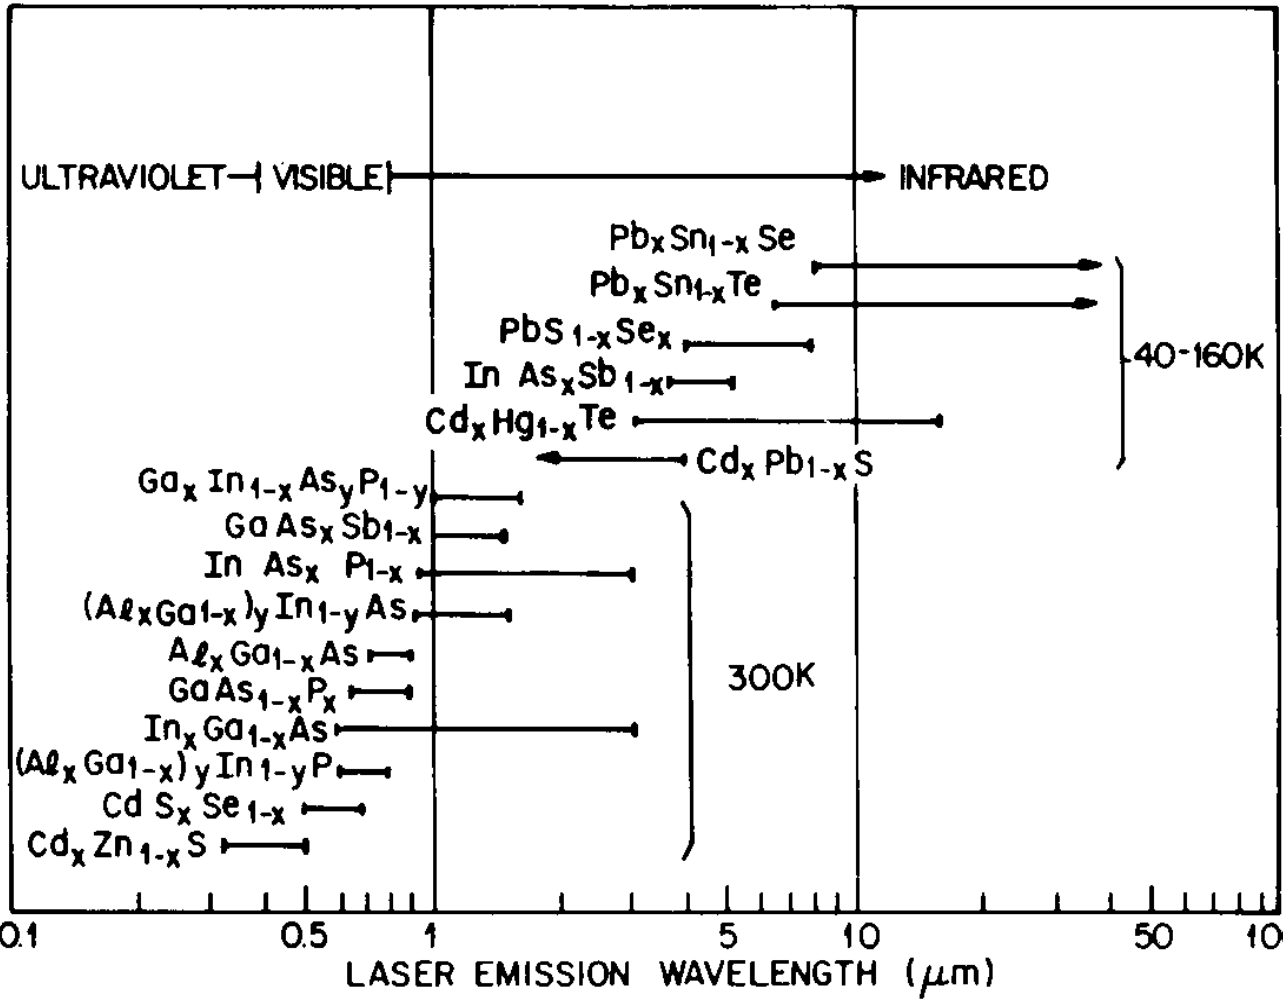
\includegraphics[width=0.5\linewidth]{../assets/laser_materials.png}
	\caption{Laser emission wavelength ranges for different semiconductor material
	systems, separated into room-temperature (\qty{300}{\kelvin}) and low-temperature
	(\qtyrange{40}{60}{\kelvin}{40}{unit}). \imcite{sze_physics_2021}. }
	\label{fig:laser_materials}
\end{figure}